\documentclass[border=3pt]{standalone}
% Preâmbulo compartilhado pelos diagramas TikZ da aula 6 de IHC (Necessidades e Requisitos)
\usepackage[T1]{fontenc}
\usepackage[utf8]{inputenc}
\usepackage{lmodern}
\usepackage{amsmath}
\usepackage{xcolor}
\usepackage{tikz}
\usetikzlibrary{arrows.meta,angles,quotes,decorations.pathmorphing,calc,
                positioning,shapes.geometric,shapes.misc,backgrounds,fit,
                math}

% Paleta (mesma dos SVGs originais)
% Paleta da disciplina de IHC: acento roxo (#755099), da capa do livro.
% (o nome "dblue" é mantido para não alterar todos os diagramas)
\definecolor{dblue}{HTML}{755099}
\definecolor{dorange}{HTML}{B3541E}
\definecolor{dgreen}{HTML}{4A7C59}
\definecolor{dred}{HTML}{9C4B4B}
\definecolor{dcream}{HTML}{F4F1EA}
\definecolor{dshade}{HTML}{DDD7C9}

% Função gaussiana (não normalizada por padrão de escala visual)
\pgfmathdeclarefunction{gauss}{3}{%
  \pgfmathparse{1/(#3*sqrt(2*pi))*exp(-((#1-#2)^2)/(2*#3^2))}%
}

% Estilos comuns (prefixo d... para não colidir com chaves internas do pgf)
\tikzset{
  >={Stealth[length=2mm]},
  dguide/.style={gray!55, dashed, line width=0.4pt},
  daxis/.style={gray!60, line width=0.7pt, ->},
  dbody/.style={fill=black!3, draw=black!80, line width=1pt},
  dacc/.style={draw=dblue, line width=1pt},
  dlbl/.style={black!55, font=\small},
  dsub/.style={black!45, font=\footnotesize},
  dstate/.style={circle, draw=black!80, fill=dcream, line width=1pt,
                 minimum size=17mm, font=\large, inner sep=1pt},
  dobs/.style={circle, draw=black!80, fill=dshade, line width=1pt,
               minimum size=14mm, font=\large, inner sep=1pt},
  dbox/.style={rounded corners=2pt, draw=black!80, fill=dcream, line width=1pt,
               align=center, inner sep=6pt},
  dop/.style={circle, draw=black!80, fill=white, line width=1pt,
              minimum size=6mm, inner sep=0pt, font=\small},
  dtrans/.style={->, dblue, line width=1pt},
  dmeas/.style={->, dorange, line width=1pt},
  dcurve/.style={line width=1pt, dblue},
  dcurveb/.style={line width=1.4pt, dorange},
}

\begin{document}
\hyphenpenalty=10000 \exhyphenpenalty=10000 \tolerance=9999 \emergencystretch=3em
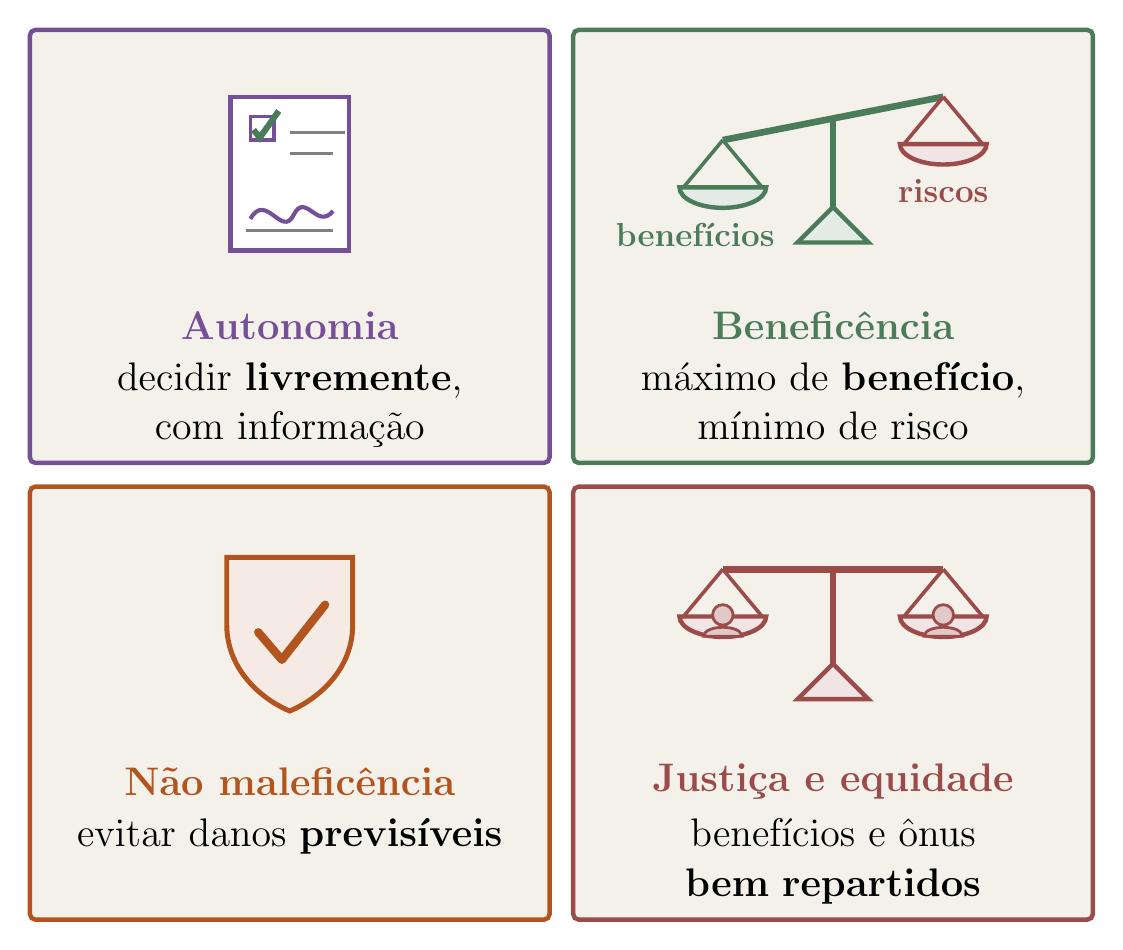
\begin{tikzpicture}[x=1cm,y=1cm]
\node[dbox, draw=dblue, line width=1.6pt, minimum width=6.6cm, minimum height=5.5cm] at (3.30,8.55) {};
\node[font=\Large\bfseries, dblue] at (3.30,7.55) {Autonomia};
\node[font=\Large, text width=6.0cm, align=center, anchor=north] at (3.30,7.20) {decidir \textbf{livremente}, com informação};
\draw[dblue, fill=white, line width=1.6pt] (2.55,8.50) rectangle (4.05,10.45);
\draw[dblue, line width=1.3pt] (2.80,9.90) rectangle ++(0.3,0.3);
\draw[dgreen, line width=2.2pt] (2.84,10.03) -- (2.92,9.93) -- (3.16,10.27);
\draw[black!50, line width=1.1pt] (3.30,10.00) -- ++(0.7,0) (3.30,9.73) -- ++(0.55,0);
\draw[dblue, line width=1.5pt] (2.80,8.90) .. controls (3.00,9.25) and (3.20,8.65) .. (3.35,8.95) .. controls (3.50,9.25) and (3.65,8.75) .. (3.85,9.00);
\draw[black!50, line width=1pt] (2.75,8.75) -- ++(1.1,0);
\node[dbox, draw=dgreen, line width=1.6pt, minimum width=6.6cm, minimum height=5.5cm] at (10.20,8.55) {};
\node[font=\Large\bfseries, dgreen] at (10.20,7.55) {Beneficência};
\node[font=\Large, text width=6.0cm, align=center, anchor=north] at (10.20,7.20) {máximo de \textbf{benefício}, mínimo de risco};
\draw[dgreen, line width=2pt] (10.20,8.60) -- (10.20,10.20);
\draw[dgreen, line width=1.6pt, fill=dgreen!15!white] (9.75,8.60) -- (10.65,8.60) -- (10.20,9.05) -- cycle;
\draw[dgreen, line width=2.4pt] (8.80,9.90) -- (11.60,10.45);
\draw[dgreen, line width=1.3pt] (8.80,9.90) -- (8.30,9.30) (8.80,9.90) -- (9.30,9.30);
\draw[dgreen, line width=1.6pt, fill=dgreen!15!white] (8.25,9.30) arc (180:360:0.55 and 0.26) -- cycle;
\draw[dred, line width=1.3pt] (11.60,10.45) -- (11.10,9.85) (11.60,10.45) -- (12.10,9.85);
\draw[dred, line width=1.6pt, fill=dred!15!white] (11.05,9.85) arc (180:360:0.55 and 0.26) -- cycle;
\node[font=\large\bfseries, dgreen] at (8.45,8.70) {benefícios};
\node[font=\large\bfseries, dred] at (11.60,9.25) {riscos};
\node[dbox, draw=dorange, line width=1.6pt, minimum width=6.6cm, minimum height=5.5cm] at (3.30,2.75) {};
\node[font=\Large\bfseries, dorange] at (3.30,1.75) {Não maleficência};
\node[font=\Large, text width=6.0cm, align=center, anchor=north] at (3.30,1.40) {evitar danos \textbf{previsíveis}};
\draw[dorange, fill=dorange!12!white, line width=1.8pt] (2.50,4.60) -- (4.10,4.60) -- (4.10,3.75) .. controls (4.10,3.10) and (3.55,2.75) .. (3.30,2.65) .. controls (3.05,2.75) and (2.50,3.10) .. (2.50,3.75) -- cycle;
\draw[dorange, line width=3pt, line cap=round, line join=round] (2.90,3.65) -- (3.20,3.30) -- (3.75,4.00);
\node[dbox, draw=dred, line width=1.6pt, minimum width=6.6cm, minimum height=5.5cm] at (10.20,2.75) {};
\node[font=\Large\bfseries, dred] at (10.20,1.75) {Justiça e equidade};
\node[font=\Large, text width=6.0cm, align=center, anchor=north] at (10.20,1.40) {benefícios e ônus \textbf{bem repartidos}};
\draw[dred, line width=2pt] (10.20,2.80) -- (10.20,4.45);
\draw[dred, line width=1.6pt, fill=dred!15!white] (9.75,2.80) -- (10.65,2.80) -- (10.20,3.25) -- cycle;
\draw[dred, line width=2.4pt] (8.80,4.45) -- (11.60,4.45);
\draw[dred, line width=1.3pt] (8.80,4.45) -- (8.30,3.85) (8.80,4.45) -- (9.30,3.85);
\draw[dred, line width=1.6pt, fill=dred!15!white] (8.25,3.85) arc (180:360:0.55 and 0.26) -- cycle;
\draw[dred, line width=1.3pt] (11.60,4.45) -- (11.10,3.85) (11.60,4.45) -- (12.10,3.85);
\draw[dred, line width=1.6pt, fill=dred!15!white] (11.05,3.85) arc (180:360:0.55 and 0.26) -- cycle;
\fill[dred!30!white, draw=dred, line width=1pt] (8.80,3.87) circle (0.13);
\fill[dred!30!white, draw=dred, line width=1pt] (8.56,3.60) .. controls (8.56,3.75) and (9.04,3.75) .. (9.04,3.60) -- cycle;
\fill[dred!30!white, draw=dred, line width=1pt] (11.60,3.87) circle (0.13);
\fill[dred!30!white, draw=dred, line width=1pt] (11.36,3.60) .. controls (11.36,3.75) and (11.84,3.75) .. (11.84,3.60) -- cycle;
\end{tikzpicture}
\end{document}
